This just in\ldots{}

\begin{figure}
\centering
\pandocbounded{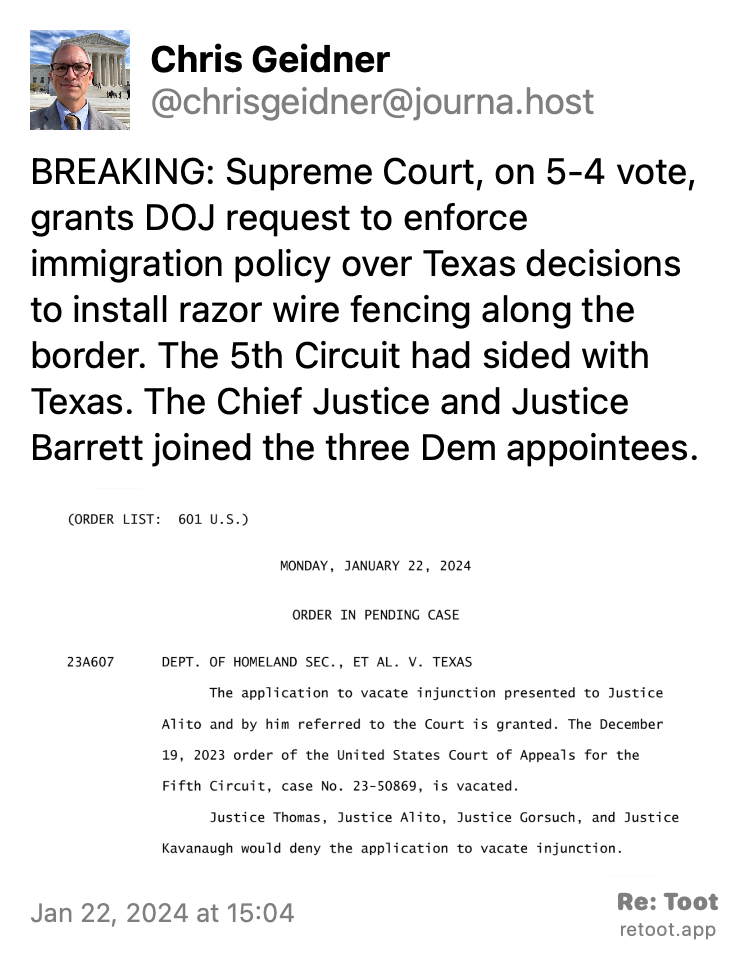
\includegraphics[keepaspectratio]{\%7B\%7Bsite.url\%7D\%7D/img/injunction-dissolved.jpg}}
\caption{Post by Chris Geidner. ``BREAKING: Supreme Court, on 5-4 vote,
grants DOJ request to enforce immigration policy over Texas decisions to
install razor wire fencing along the border. The 5th Circuit had sided
with Texas. The Chief Justice and Justice Barrett joined the three Dem
appointees.'' The post contains an image with the following description:
``(ORDER LIST: 601 U.S.) MONDAY, JANUARY 22, 2024 ORDER IN PENDING CASE
23A607 DEPT. OF HOMELAND SEC., ET AL. V. TEXAS The application to vacate
injunction presented to Justice Alito and by him referred to the Court
is granted. The December 19, 2023 order of the United States Court of
Appeals for the Fifth Circuit, case No.~23-50869, is vacated. Justice
Thomas, Justice Alito, Justice Gorsuch, and Justice Kavanaugh would deny
the application to vacate injunction.'' Posted on Jan 22, 2024 at 15:04}
\end{figure}

Quoting
\href{https://journa.host/@chrisgeidner/}{@chrisgeidner@journa.host}:
\url{https://journa.host/@chrisgeidner/111801394159140607} \#retoot

\begin{quote}
\emph{Post by Chris Geidner. ``BREAKING: Supreme Court, on 5-4 vote,
grants DOJ request to enforce immigration policy over Texas decisions to
install razor wire fencing along the border. The 5th Circuit had sided
with Texas. The Chief Justice and Justice Barrett joined the three Dem
appointees.'' The post contains an image with the following description:
``(ORDER LIST: 601 U.S.) MONDAY, JANUARY 22, 2024 ORDER IN PENDING CASE
23A607 DEPT. OF HOMELAND SEC., ET AL. V. TEXAS The application to vacate
injunction presented to Justice Alito and by him referred to the Court
is granted. The December 19, 2023 order of the United States Court of
Appeals for the Fifth Circuit, case No.~23-50869, is vacated. Justice
Thomas, Justice Alito, Justice Gorsuch, and Justice Kavanaugh would deny
the application to vacate injunction.'' Posted on Jan 22, 2024 at 15:04}
\end{quote}

I've yelled at my local congressman to remind him that he too is a
border congressman. He just happens to represent the \emph{northern}
border that touches Canada's border line out in the middle of Lake Erie.
Ashtabula County literally borders Elgin and Norfolk counties of
Canada's Ontario province.

Texas was doing some crazy and inhuman things out there. Texas militia
on state mission orders was clashing with federal forces. Texas was
raising some crazy arguments under
\href{https://constitution.congress.gov/browse/article-1/section-10/clause-3/}{Clause
3 of Section 10 of Article I of the federal constitution} which states:

\begin{quote}
\emph{No State shall, without the Consent of Congress, lay any Duty of
Tonnage, keep Troops, or Ships of War in time of Peace, enter into any
Agreement or Compact with another State, or with a foreign Power, or
engage in War, unless actually invaded, or in such imminent Danger as
will not admit of delay.}
\end{quote}

The main argument Texas has been making is that it thinks it is
``actually invaded'' and that it can therefore proceed with war-like
acts without the federal government's consent as it tries to beat back
the supposed invader. They lost on that argument in the original trial.
When they went on appeal to the United States Court of Appeals for the
Fifth Circuit they got an injunction that effectively breathed life back
into their argument. The Chief Justice and justices Barrett, Sotomayor,
Kagan, and Jackson nuked the injunction.

The Republican Party is exceedingly fixated on the southern border. The
governors of Texas and Florida have been using it to cause an interstate
crisis by shipping migrants around the country. This legal battles
creates a further flashpoint.

I've referred to the events of the 2021 coup attempt by the cultists as
being akin to
\href{https://www.nps.gov/articles/john-browns-raid.htm}{John Brown's
raid on Harpers Ferry}. It wasn't the main event. It was only a prelude.
Are we looking at something in Texas where things may kick off? When you
have uniformed state militia preventing federal employees and federal
law enforcement from doing their jobs as we've already seen at Eagle
Park, you're not that far away from something stupid happening.

The next big event is the primary Tuesday in New Hampshire. Nikki Haley
has to win it or the Republican primary is basically over. If the vote
turns out in keeping with opinion polls, we're possibly going to see her
drop out in short order.

Remember what I wrote a few days ago about lived horror? Generally it
starts slowly. The pace picks up fairly quickly.

The deepfake calls copying President Biden's voice urging voters in New
Hampshire to not vote on Tuesday are only the beginning of AI-fueled
chaos this year, I think\ldots{}
